\documentclass{standalone}
\usepackage{tikz}
\usetikzlibrary{arrows}
\usetikzlibrary{positioning}
\usetikzlibrary{shapes.geometric}
\usepackage{amsmath}
\begin{document}
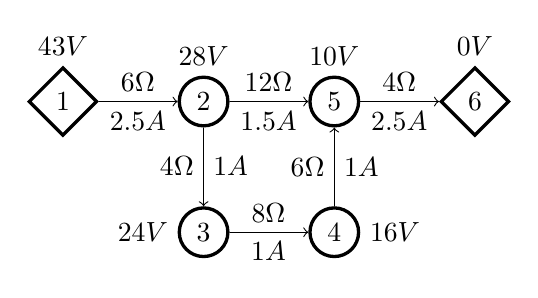
\begin{tikzpicture}[
endnode/.style={diamond, draw=black, fill=none, very thick, minimum size=1em},
node/.style={circle, draw=black, fill=none, very thick, minimum size=1em},
]
\node[endnode, label={$43V$}](n1){1};
\node[node, label={$28V$}](n2)[right=of n1]{2};
\node[node, label=left:{$24V$}](n3)[below=of n2]{3};
\node[node, label=right:{$16V$}](n4)[right=of n3]{4};
\node[node, label={$10V$}](n5)[right=of n2]{5};
\node[endnode, label={$0V$}](n6)[right=of n5]{6};
\draw[->] (n1.east) -- node[above]{$6\Omega$}++(0.99,0) -- node{}++(-0.99,0) -- node[below]{$2.5A$}++(0.99,0) -- (n2.west);
\draw[->] (n2.east) -- node[above]{$12\Omega$}++(0.99,0) -- node{}++(-0.99,0) -- node[below]{$1.5A$}++(0.99,0) -- (n5.west);
\draw[->] (n5.east) -- node[above]{$4\Omega$}++(0.99,0) -- node{}++(-0.99,0) -- node[below]{$2.5A$}++(0.99,0) -- (n6.west);
\draw[->] (n2.south) -- node[left]{$4\Omega$}++(0,-0.99) -- node{}++(0,0.99) -- node[right]{$1A$}++(0,-0.99) -- (n3.north);
\draw[->] (n3.east) -- node[above]{$8\Omega$}++(0.99,0) -- node{}++(-0.99,0) -- node[below]{$1A$}++(0.99,0) -- (n4.west);
\draw[->] (n4.north) -- node[left]{$6\Omega$}++(0,0.99) -- node{}++(0,-0.99) -- node[right]{$1A$}++(0,0.99) -- (n5.south);
\end{tikzpicture}
\end{document}

